\chapter{評估與結果}

\section{結果呈現}
\subsection{Github Page}
本組專題成果網頁係藉由藉由本組指導教授嚴家銘教授所開發的cmsimde子模組進行維護。\\

\begin{figure}[h]
    \centering
    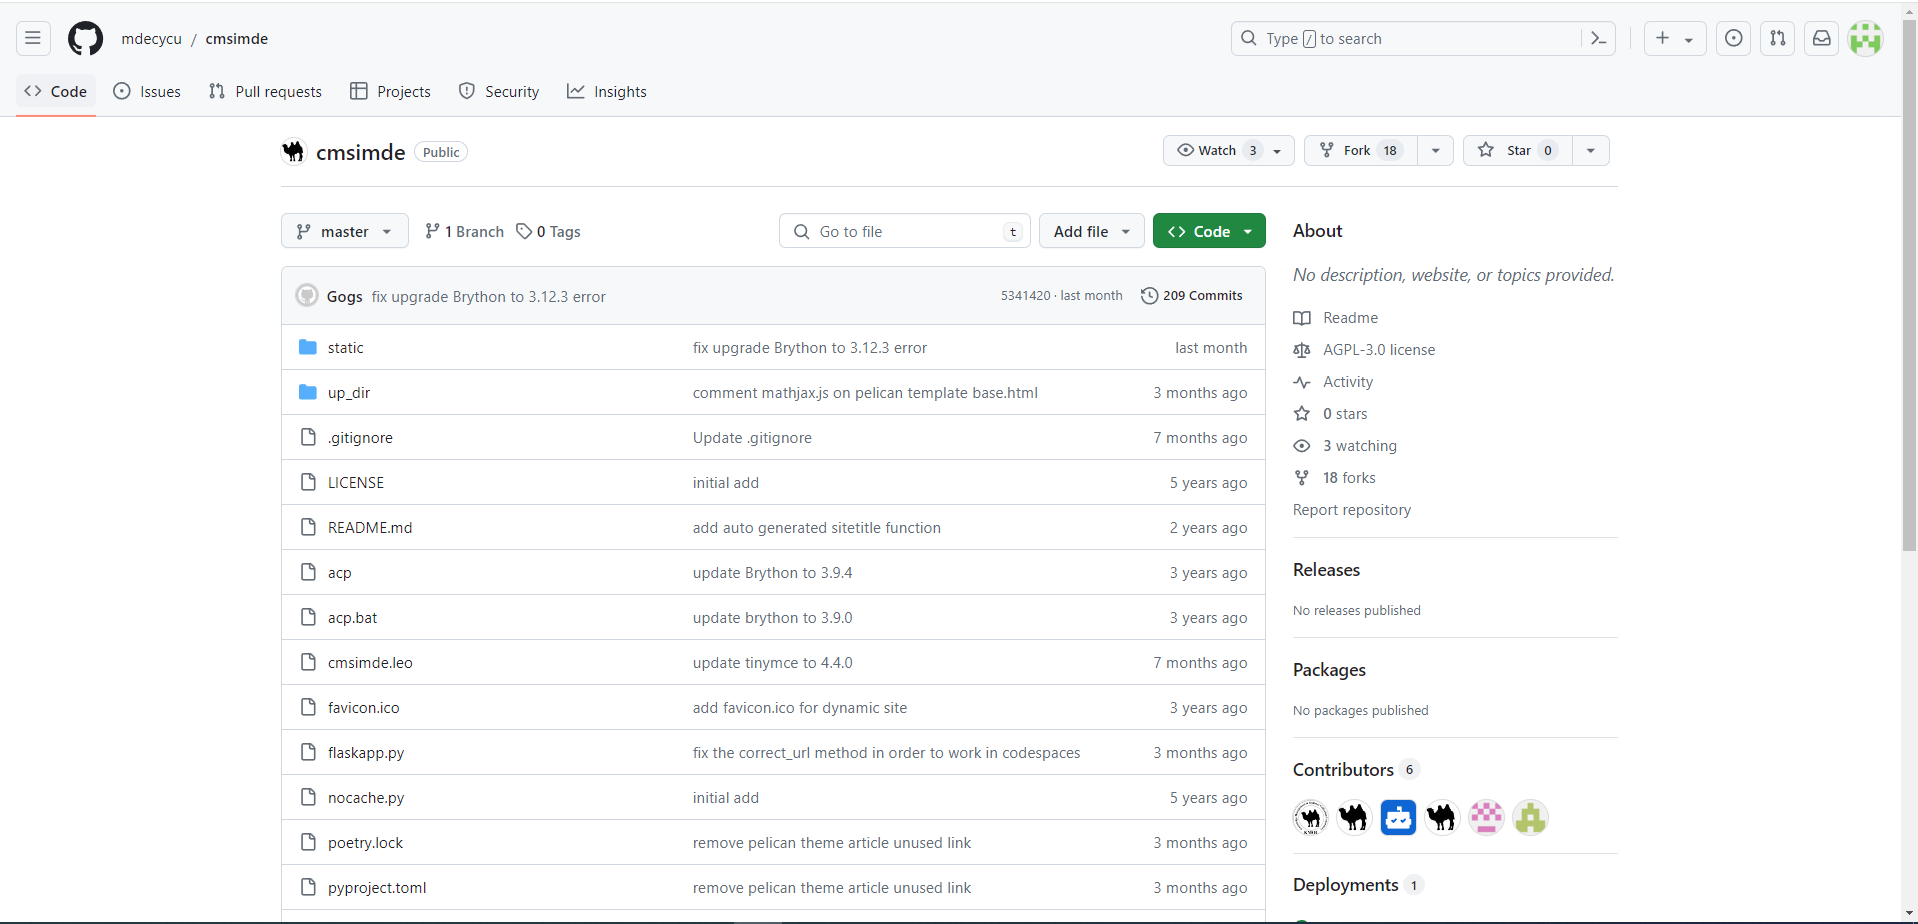
\includegraphics[width=0.8\textwidth]{cmsimde}
    \caption{cmsimde}
\end{figure}

組員只要在可攜環境的近端倉內使用終端機執行cms.bat,就會以python運行cmsimde資料夾中的wsgi.py,
接著就會透過flaskapp.py等檔案啟動近端的動態網頁。
組員即可透過瀏覽器編輯動態網頁,編輯完成後亦可透過編輯器內的選項將動態網頁轉換為靜態,並推送至Github倉儲中,由遠端倉儲生成網頁,
網址為\url{https://mde.tw/pj4101}。\\

\begin{figure}[h]
    \centering
    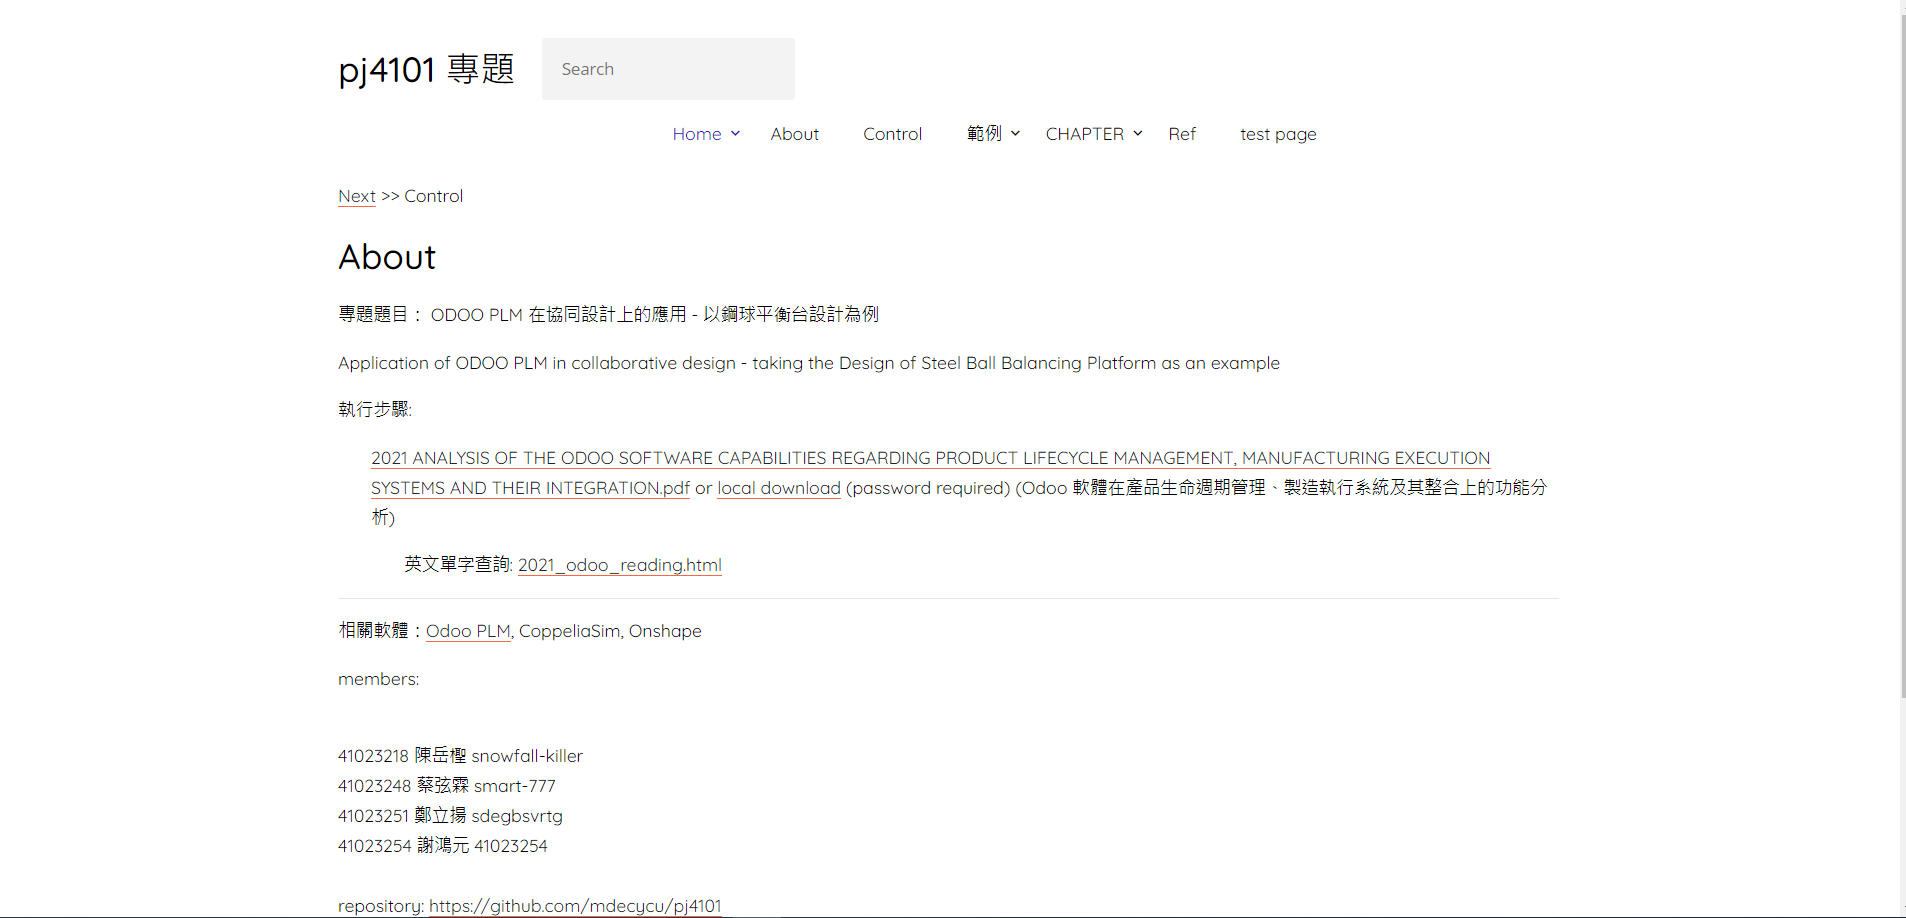
\includegraphics[width=0.8\textwidth]{mdepj4101}
    \caption{本組專題網頁}
\end{figure}

在此環境之下,本組組員能非常輕鬆的協同對網頁進行維護。\\

\subsection{Repository}
由於協同需求,本組採用Github倉儲作為報告檔案
\begin{figure}[h]
    \centering
    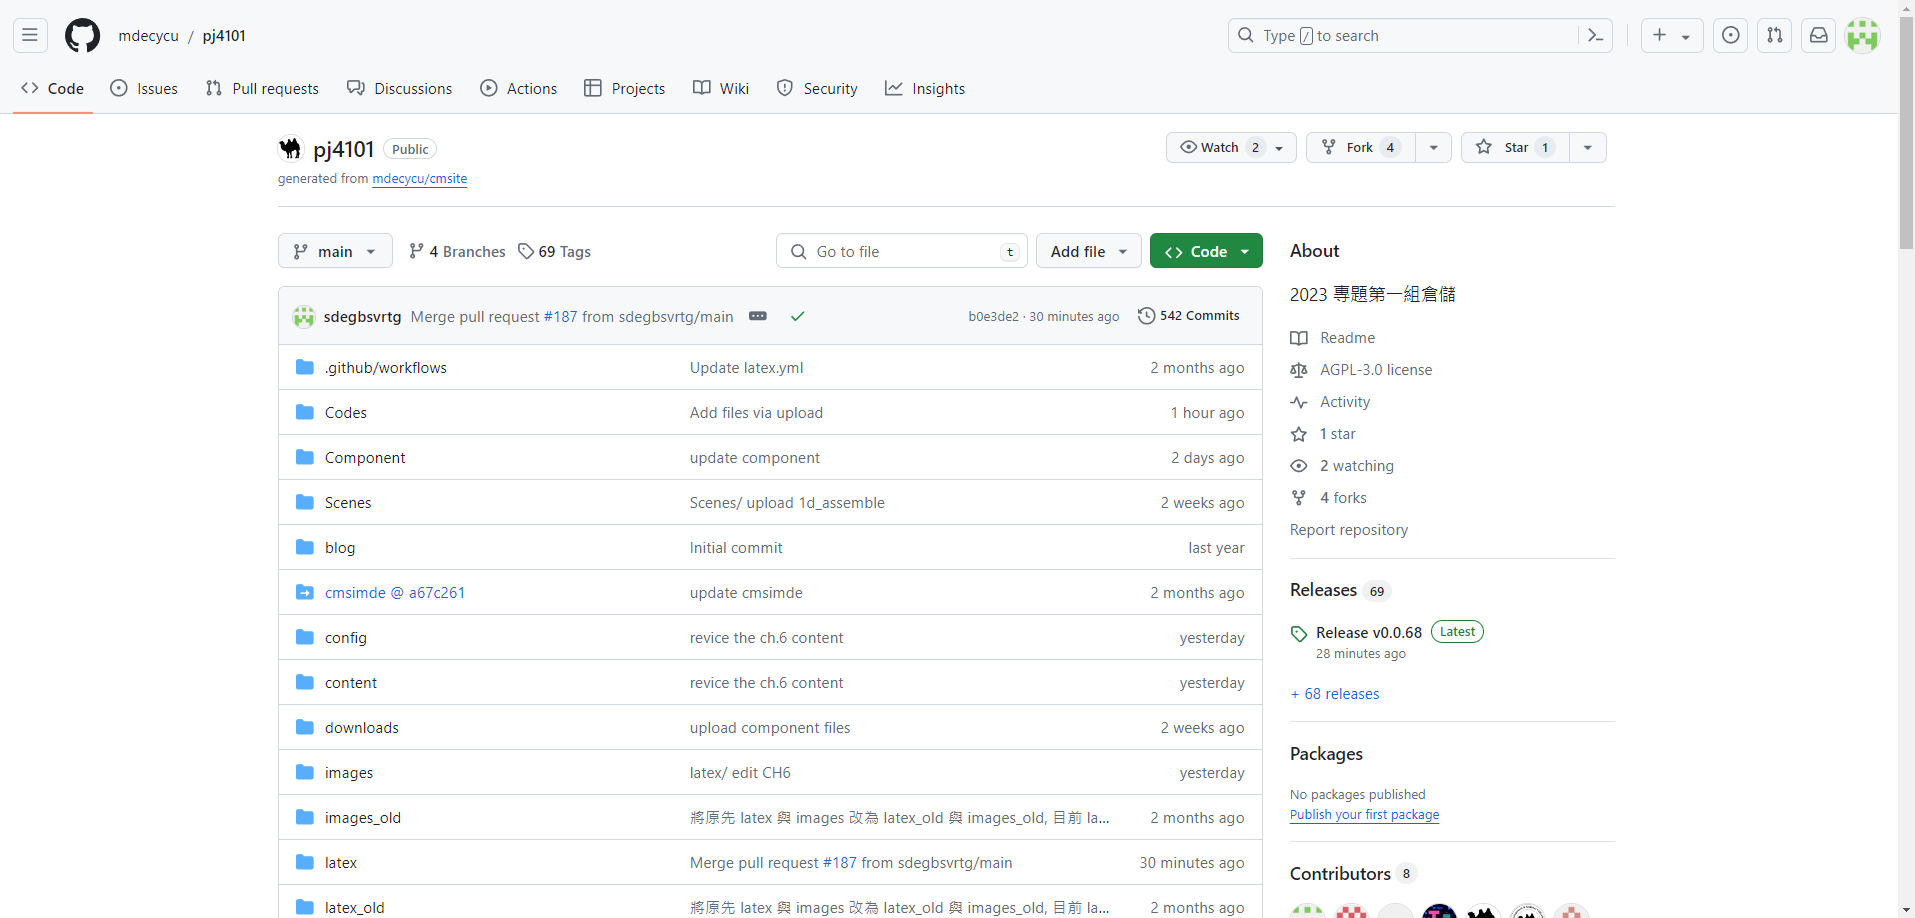
\includegraphics[width=0.8\textwidth]{repo}
    \caption{本組專題倉儲}
\end{figure}

\subsection{PID}
38.5
5
31.5

\subsection{}

\section{結果分析}
\subsection{}
\subsection{}
\subsection{}

\section{討論}
\subsection{}
\subsection{}
\subsection{}